% !TEX program = pdflatex
% ============================================================
% Semantic segmentation in remote sensing — general-purpose talk
% after M. Pastorino, G. Moser, J. Zerubia
% (../../article/Martina_TSI_GRETSI_segmentation_semantique.pdf).
%
% English version of ../main.tex: same theme, same content, same
% 51 slides. The only deliberate difference is the language.
%
% Meant for general use (seminar, course, invited talk): no conference
% and no date anywhere on the slides.
%
% The presentation follows the structure of the paper (11 sections).
% Illustrations: the figures of the paper, extracted in imgs/article/;
% credits below the sub-captions and a "Figure credits" back-up slide.
%
% Build: make  (latexmk + pdfLaTeX + biber, theme in theme/)
% ============================================================
\documentclass[svgnames,9pt,aspectratio=169]{beamer}

\usepackage[english]{babel}
\usepackage{csquotes}
\usepackage{amsmath,amssymb,amsfonts,mathtools}
\usepackage{graphicx}
\usepackage{booktabs}
\usepackage{tikz}
\usetikzlibrary{positioning, shapes, arrows.meta, calc, fit, backgrounds, babel}

% ------------------------------------------------------------
% The theme tests the \draftmode primitive. LuaTeX provides it; pdfTeX
% has only known it since TeX Live 2024 (it was \pdfdraftmode before).
% This alias lets the file compile with either engine.
% ------------------------------------------------------------
\makeatletter
\ifdefined\draftmode\else
  \ifdefined\pdfdraftmode
    \let\draftmode\pdfdraftmode
  \else
    \providecommand{\draftmode}{0}%
  \fi
\fi
\makeatother

% ------------------------------------------------------------
% Inria 2024 Beamer theme (theme/ directory, unmodified).
% ------------------------------------------------------------
\usetheme{inria}
\renewcommand{\thankyou}{Thank you for your attention.}

% ------------------------------------------------------------
% Bibliography: the order of the .bib file is the order of the paper.
% \nocite{*} appears at the start of the document so that the [n]
% numbers on the slides follow that order.
% ------------------------------------------------------------
\usepackage[backend=biber,style=numeric,sorting=none,
            maxbibnames=4,minbibnames=3,giveninits=true,
            doi=false,isbn=false,url=false,eprint=false]{biblatex}
\addbibresource{references.bib}
\renewcommand*{\bibfont}{\tiny}
\setlength{\bibitemsep}{0.35ex}

% ------------------------------------------------------------
% Università di Genova logo (the Inria theme allows for one logo only).
% textpos coordinates: fractions of \paperwidth / \paperheight.
% ------------------------------------------------------------
\newcommand{\logounige}[1][0.185]{%
  \begin{textblock}{#1}[1,0](0.955,0.085)
    
\includegraphics[width=\textwidth]{imgs/logos/logo_orizzontale_COLORE}
  \end{textblock}}

% ------------------------------------------------------------
% Formatting commands
% ------------------------------------------------------------
% Emphasis
\newcommand{\hl}[1]{\textcolor{inria-rouge}{\textbf{#1}}}

% Inline bibliographic pointer: [n] in grey
\newcommand{\refc}[1]{\,\textcolor{gris_fonce_inria}{\footnotesize\cite{#1}}}

% Short caption under a figure (centred)
\newcommand{\legende}[1]{%
  \par\vspace{0.4ex}{\scriptsize\color{gris_fonce_inria}\centering #1\par}}

% Credit / copyright: in the flow, right below the sub-captions (centred)
\newcommand{\credit}[1]{%
  \par\vspace{0.35ex}{\tiny\color{gris_fonce_inria}\centering #1\par}}

% Full references cited on the slide, at the very bottom.
% Compact format: at most two authors, no volume, no number, no pages.
\newtoggle{brefcite}
\AtEveryCitekey{\iftoggle{brefcite}%
  {\clearfield{pages}\clearfield{volume}\clearfield{number}}{}}
\newcommand{\bibline}[1]{%
  \par\hangindent=1.1em\hangafter=1\relax
  \mbox{\cite{#1}}~%
  \AtNextCite{\toggletrue{brefcite}%
    \defcounter{maxnames}{2}\defcounter{minnames}{1}}%
  \fullcite{#1}}
\newcommand{\biblio}[1]{%
  \begin{textblock}{0.92}[0,1](0.045,0.922)%
    \begingroup
    \fontsize{4.7}{5.2}\selectfont\raggedright\color{gris_fonce_inria}%
    \setlength{\parindent}{0pt}%
    \forcsvlist{\bibline}{#1}%
    \par                       % before \endgroup: otherwise the last line
    \endgroup                  % inherits the body leading of the slide
  \end{textblock}}

% Formula box: Inria red rule, very light grey background
\newcommand{\formulebox}[2][0.80]{%
  \begin{center}%
    \setlength{\fboxrule}{0.7pt}\setlength{\fboxsep}{7pt}%
    \fcolorbox{inria-rouge}{gris_fonce_inria!6}{%
      \begin{minipage}{#1\textwidth}\centering #2\end{minipage}}%
  \end{center}}

% Running thread of the paper: progressive integration of context.
% Optional argument: number of the step to highlight (0 = none).
\newcommand{\filrouge}[1][0]{%
  \begin{center}
  \begin{tikzpicture}[x=1mm,y=1mm,font=\scriptsize\bfseries]
    \foreach \i/\c/\t in {%
        0/inria-2024-bleu-azur/{Local spectral\\information},
        1/inria-2024-bleu-canard/{Spatial\\coherence},
        2/inria-2024-bleu-nuit/{Boundaries,\\regions, objects},
        3/inria-2024-violet/{Representation\\learning},
        4/inria-2024-rouge/{Foundation\\models}}
      {%
        \node[fill=\c,text=white,align=center,text width=19mm,
              minimum height=11mm,inner sep=1.5pt] at ({\i*23},0) {\t};
        \ifnum\i>0
          \draw[-{Latex[length=1.8mm]},line width=0.8pt,gris_fonce_inria]
                ({\i*23-13},0) -- ({\i*23-10},0);
        \fi
      }
  \end{tikzpicture}
  \end{center}}

% Slightly airier lists, sub-items indented a little
% (the theme sets \leftmarginii and \leftmarginiii to 0pt).
\setbeamertemplate{itemize/enumerate body begin}{\setlength{\itemsep}{0.85ex}}
\setbeamertemplate{itemize/enumerate subbody begin}{\setlength{\itemsep}{0.35ex}}
\setlength{\leftmarginii}{1.4em}
\setlength{\leftmarginiii}{1.4em}

% Table of contents
\addto\captionsenglish{\renewcommand{\contentsname}{Outline}}

% ------------------------------------------------------------
% Metadata
% ------------------------------------------------------------
% Neutralises the formatting of the affiliation block when hyperref
% turns \author into a PDF string.
\makeatletter
\pdfstringdefDisableCommands{%
  \let\textsc\@firstofone
  \let\emph\@firstofone
  \let\cite\@gobble
  \let\textsuperscript\@gobble
  \def\,{ }%
  \def\\{ }%
}
\makeatother

% NB: affiliations to be confirmed before circulation.
\title{Semantic segmentation in remote sensing}
\subtitle{After the survey paper~\cite{pastorino2026segmentation}}
% The theme prints the optional argument of \date in the footer. We put the
% short title there rather than a conference or a date, so that the deck can be
% used as is on any occasion.
\date[Semantic segmentation in remote sensing]{}
\author{%
   Josiane \textsc{Zerubia}\\[2pt]
   \footnotesize Inria Centre at Université Côte d'Azur, \textsc{Ayana} project-team\\[8pt]
   \footnotesize in collaboration with Martina \textsc{Pastorino} and Gabriele \textsc{Moser}\\
   \footnotesize Università di Genova, \textsc{Diten}%
}
\institute{Sophia Antipolis}

\hypersetup{
   allcolors   = rouge_inria,
   pdfauthor   = {Josiane Zerubia, in collaboration with Martina Pastorino and Gabriele Moser},
   pdftitle    = {Semantic segmentation in remote sensing},
   pdfsubject  = {Talk after the survey paper by M. Pastorino, G. Moser and J. Zerubia},
   pdfkeywords = {semantic segmentation, remote sensing, Markov random fields, CRF,
                  variational methods, deep learning, foundation models}
}

% ============================================================
\begin{document}
\nocite{*}   % freezes the [n] numbering to the order of the .bib file

% ---- Title page --------------------------------------------
\frame{%
  \titlepage
  \logounige
  \biblio{pastorino2026segmentation}
}

% ---- Outline -----------------------------------------------
\begin{frame}{Outline}
  \begin{columns}[T,onlytextwidth]
    \begin{column}{0.49\textwidth}
      \tableofcontents[sections={1-6}]
    \end{column}
    \begin{column}{0.49\textwidth}
      \tableofcontents[sections={7-11}]
    \end{column}
  \end{columns}
\end{frame}

% ============================================================
\section{Introduction}
% ============================================================
\frame{\sectionpage}

\begin{frame}{From image to thematic map}
  \begin{itemize}
    \item Assign to \hl{every pixel} a label from a predefined set of semantic
          classes\refc{duda1973pattern}\refc{swain1978remote}\refc{richards1986remote}:
          a problem studied for decades under the names \emph{supervised},
          \emph{per-pixel} and \emph{contextual} classification
    \item Produces a \hl{dense map}, to be distinguished from segmentation, which partitions
          the image into homogeneous regions \emph{without} attaching any meaning to them
    \item In remote sensing: turning satellite observations into
          \hl{land-cover and land-use maps}
  \end{itemize}
  \vspace{0.4ex}
  % Two minipages centered together: thumbnails moved closer and enlarged,
  % each keeping its own subcaption (review request).
  \centerline{%
    \begin{minipage}[t]{0.22\textwidth}\centering
      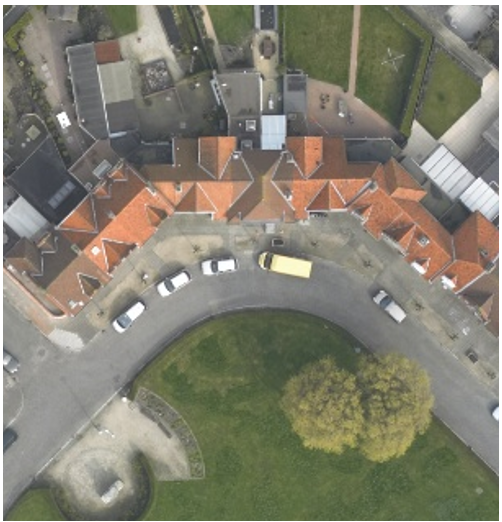
\includegraphics[height=2.0cm]{imgs/article/fig1a_zeebruges_image_aerienne}
      \legende{(a) aerial image}
    \end{minipage}\hspace{3mm}%
    \begin{minipage}[t]{0.22\textwidth}\centering
      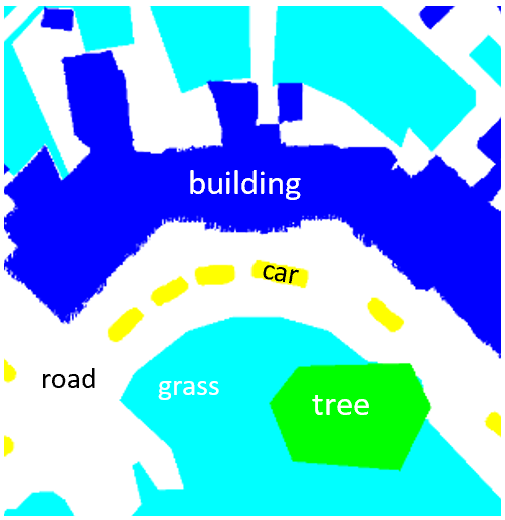
\includegraphics[height=2.0cm]{imgs/article/fig1b_zeebruges_carte_segmentation}
      \legende{(b) segmentation map}
    \end{minipage}}
  \credit{\emph{Zeebruges} dataset, IEEE GRSS IADF Technical Committee;
    imagery and ground truth: Belgian Royal Military Academy and ONERA.}
  \biblio{duda1973pattern,swain1978remote,richards1986remote}
\end{frame}

\begin{frame}{What sets remote sensing apart}
  \begin{itemize}
    \item Heterogeneous \hl{sensors}: optical, synthetic aperture radar (SAR),
          LiDAR
    \item Widely varying \hl{spatial resolutions}, acquisitions at
          \hl{different dates}, \hl{several modalities} combined
    \item \hl{Complex geographical scenes} whose properties vary with region,
          season and acquisition conditions
    \item Consequence: the evolution of the field \hl{is not} a mere \hl{adaptation}
          of advances in \hl{computer vision}
    \item It is a convergence between \hl{statistical pattern recognition},
          \hl{signal and image processing}, \hl{probabilistic modeling},
          \hl{mathematical morphology}, \hl{stochastic geometry},
          \hl{object-based image analysis} and, recently, \hl{deep learning}
  \end{itemize}
\end{frame}

\begin{frame}{Formalization and storyline}
  \formulebox{$I : \Omega \longrightarrow \mathbb{R}^{d}
              \qquad\text{then}\qquad
              f : \Omega \longrightarrow \mathcal{C}$}
  \begin{itemize}
    \item $\Omega$: the image domain; $d$: the number of variables (panchromatic
          band, multispectral or hyperspectral bands, SAR polarizations,
          LiDAR measurements, spectral indices, digital terrain models\dots)
    \item $\mathcal{C}$: the finite set of semantic classes
    \item \hl{The storyline of this talk}: the progressive integration of
          increasing levels of context
  \end{itemize}
  \vspace{0.4ex}
  \filrouge
\end{frame}

% ============================================================
\section{Per-pixel statistical classification}
% ============================================================
\frame{\sectionpage}

\begin{frame}{The first approaches (1970s--1980s)}
  \begin{itemize}
    \item Landsat (optical) and SeaSat (radar) create the need for automatic
          land-cover maps\refc{schowengerdt2007remote}\refc{landgrebe2003signal}\refc{ulaby2015microwave}
    \item Each pixel is an observation vector
          $\mathbf{x} = (x_1,\dots,x_d)^{\mathsf{T}}$: radiometric responses,
          SAR intensities, indices, ancillary data\refc{duda1973pattern}
  \end{itemize}
  \formulebox{$\hat{\omega} \;=\; \arg\max_{\omega_i}\; P(\omega_i \mid \mathbf{x})$}
  \begin{itemize}
    \item Under a multivariate Gaussian assumption: the \hl{MAP classifier},
          \enquote{maximum a posteriori}, the reference method for several
          decades\refc{swain1978remote}\refc{richards1986remote}\refc{mather2004computer}
  \end{itemize}
  \biblio{duda1973pattern,swain1978remote,richards1986remote,schowengerdt2007remote,landgrebe2003signal,ulaby2015microwave,mather2004computer}
\end{frame}

\begin{frame}{Two structural limitations}
  \begin{itemize}
    \item \hl{Curse of dimensionality} (Hughes phenomenon, described as early as
          1968)\refc{hughes1968mean}
      \begin{itemize}
        \item more spectral variables $\neq$ better performance when the number
              of training samples remains limited
        \item spectral signatures alone are not enough
      \end{itemize}
    \item \hl{Independence assumption on the observations}
      \begin{itemize}
        \item each pixel is decided in isolation, without using its neighborhood
        \item yet geographical objects are strongly spatially correlated:
              agricultural fields, forests, urban areas, road networks
      \end{itemize}
    \item Consequence: \hl{noisy maps}, all the more so as spatial resolution
          increases
  \end{itemize}
  \biblio{hughes1968mean}
\end{frame}

\begin{frame}{The result: noisy maps}
  \begin{columns}[T,onlytextwidth]
    \begin{column}{0.49\textwidth}\centering
      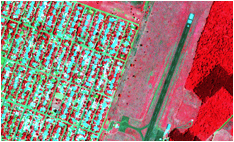
\includegraphics[width=0.72\textwidth]{imgs/article/fig2a_ikonos_fausses_couleurs}
      \legende{(a) IKONOS image, 4~m, false color}
    \end{column}
    \begin{column}{0.49\textwidth}\centering
      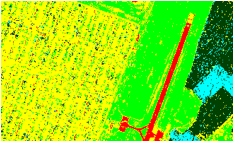
\includegraphics[width=0.72\textwidth]{imgs/article/fig2b_classification_pixel_a_pixel}
      \legende{(b) per-pixel classification}
    \end{column}
  \end{columns}
  \credit{IKONOS image, 4~m, 3 bands, false-color composite (near infrared, red,
    blue); segmentation map \cite{moser2013landcover}.}
  \vspace{0.6ex}
  \begin{itemize}
    \item The decision no longer depends on the radiometry of a single pixel
          alone: its \hl{spatial environment} is needed
    \item The problem stops being a spectral classification and becomes one of
          \hl{spatial interpretation of
          scenes}\refc{geman1984stochastic}\refc{besag1986statistical}\refc{solberg1996markov}
  \end{itemize}
  \biblio{geman1984stochastic,besag1986statistical,solberg1996markov,moser2013landcover}
\end{frame}

% ============================================================
\section{Discriminative and kernel methods}
% ============================================================
\frame{\sectionpage}

\begin{frame}{Estimating the boundary rather than the distribution}
  \begin{itemize}
    \item From the late 1990s: estimating \hl{the decision boundaries directly}
          rather than the distribution of the observations
    \item A response to two difficulties: \hl{unrealistic} Gaussian assumptions,
          \hl{high dimensionality} of the data
    \item \hl{Support vector machines (SVMs)}, arising from statistical learning
          theory\refc{vapnik1998statistical}\refc{cortes1995support}
      \begin{itemize}
        \item principle of \hl{margin maximization} between classes
        \item \hl{excellent generalization} even when the number of training
              samples is small compared with the dimension
      \end{itemize}
  \end{itemize}
  \biblio{vapnik1998statistical,cortes1995support}
\end{frame}

\begin{frame}{Kernels: nonlinearity without losing convexity}
  \begin{itemize}
    \item Kernel methods extend the framework to \hl{nonlinear} problems while
          preserving a \hl{convex formulation}\refc{scholkopf2002learning}
    \item The 2000s: SVMs become one of the \hl{most widely used} classifiers in
          remote sensing: multispectral, hyperspectral, multisource
    \item Development of \hl{kernels tailored to geospatial
          observations}\refc{campsvalls2009kernel}\refc{mountrakis2011support}
    \item \hl{But}: SVMs improve the \emph{decision function}, not the
          representation: applied to observation vectors, they remain
          \hl{per-pixel} classifiers
    \item Two research directions then evolve in parallel:
          \emph{new classifiers} and \emph{richer spatial representations}
  \end{itemize}
  \biblio{scholkopf2002learning,campsvalls2009kernel,mountrakis2011support}
\end{frame}

% ============================================================
\section{Ensemble methods}
% ============================================================
\frame{\sectionpage}

\begin{frame}{Random forests}
  \begin{itemize}
    \item Combining several classifiers to gain robustness and generalization:
          \hl{ensemble learning}
    \item \hl{Random forests}: decision trees learned on random subsets
          \emph{of the observations} and \emph{of the variables}, aggregated by
          majority vote\refc{breiman2001random}
    \item They limit overfitting while modeling nonlinear relations
    \item In practice: little tuning, robust to noise, handle a large number of
          variables, provide \hl{variable importance} measures
    \item Multispectral and hyperspectral\refc{gislason2006random}, then land
          cover, change detection, multisource data fusion\refc{belgiu2016random}
  \end{itemize}
  \biblio{breiman2001random,gislason2006random,belgiu2016random}
\end{frame}

\begin{frame}{The pixel era: takeaways}
  \begin{itemize}
    \item Discriminative and ensemble methods: clear gains \hl{on the classifier}
    \item They remain \hl{independent of the representation}, be it spectral,
          textural, morphological or spectral-spatial
    \item The fundamental limitation remains: \hl{the spatial organization of the
          scene is not taken into account explicitly}
    \item Two complementary responses will structure what follows:
      \begin{itemize}
        \item regularize the \hl{labels}: contextual, Markov,
              variational (sections 5, 6 and 8)
        \item enrich the \hl{features}: spectral-spatial, object-based
              (section 7)
      \end{itemize}
  \end{itemize}
\end{frame}

% ============================================================
\section{Contextual classification}
% ============================================================
\frame{\sectionpage}

\begin{frame}{Three levels of context}
  \begin{itemize}
    \item As early as the 1980s and 1990s: a pixel is more likely to belong to the
          class of its immediate neighbors than to another one\refc{richards1986remote}
    \item \hl{Local context}: interactions between neighboring pixels, small
          fixed-size windows\refc{haralick1985image}
    \item \hl{Regional context}: texture, shape, size, homogeneity of the segmented
          regions; foreshadows object-based image analysis\refc{blaschke2010object}
    \item \hl{Global context}: overall organization of the scene, relations between
          objects, prior knowledge about their layout
    \item A structuring hierarchy that extends to contemporary deep
          architectures\refc{azencott1992nonsupervised}\refc{csurka2023good}
  \end{itemize}
  \biblio{richards1986remote,haralick1985image,blaschke2010object,azencott1992nonsupervised,csurka2023good}
\end{frame}

\begin{frame}{The measurable contribution of context}
  \begin{columns}[T,onlytextwidth]
    \begin{column}{0.32\textwidth}\centering
      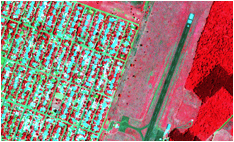
\includegraphics[width=0.84\textwidth]{imgs/article/fig2a_ikonos_fausses_couleurs}
      \legende{(a) IKONOS image}
    \end{column}
    \begin{column}{0.32\textwidth}\centering
      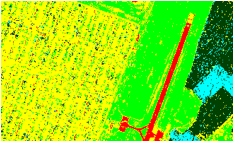
\includegraphics[width=0.84\textwidth]{imgs/article/fig2b_classification_pixel_a_pixel}
      \legende{(b) per-pixel}
    \end{column}
    \begin{column}{0.32\textwidth}\centering
      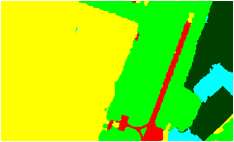
\includegraphics[width=0.84\textwidth]{imgs/article/fig2c_classification_contextuelle}
      \legende{(c) contextual}
    \end{column}
  \end{columns}
  \credit{IKONOS image, 4~m, 3 bands, false-color composite (near infrared, red,
    blue); segmentation maps \cite{moser2013landcover}.}
  \vspace{0.6ex}
  \begin{itemize}
    \item Clear gains on multispectral, multitemporal and multisource
          data\refc{solberg1996markov}\refc{bruzzone1997iterative}\refc{bruzzone1999neural}
    \item Labels are no longer decided one by one: they must be estimated
          \hl{jointly}
  \end{itemize}
  \biblio{solberg1996markov,moser2013landcover,bruzzone1997iterative,bruzzone1999neural}
\end{frame}

% ============================================================
\section{Markov and Bayesian models}
% ============================================================
\frame{\sectionpage}

\begin{frame}{Markov random fields: the first formalization}
  \begin{itemize}
    \item Labels are no longer independent: they are random variables defined on a
          \hl{neighborhood
          graph}\refc{geman1984stochastic}\refc{besag1986statistical}\refc{kato2012markov}
    \item The Markov assumptions \emph{and} the equivalence between Markov random
          fields and Gibbs distributions
  \end{itemize}
  \formulebox{$\hat{Y} \;=\; \arg\max_{Y} P(Y \mid X)
              \qquad\Longleftrightarrow\qquad
              \hat{Y} \;=\; \arg\min_{Y} U(Y \mid X)$}
  \begin{itemize}
    \item $X$: the observations; $Y$: the labels to be estimated
    \item Bayes' theorem turns MAP estimation into an
          \hl{energy minimization}
  \end{itemize}
  \biblio{geman1984stochastic,besag1986statistical,kato2012markov}
\end{frame}

\begin{frame}{Data term + regularization}
  \formulebox{$U(Y \mid X) \;=\; U_d(Y \mid X) \;+\; \beta\, U_r(Y \mid X)$}
  \begin{columns}[T,onlytextwidth]
    \begin{column}{0.56\textwidth}
      \begin{itemize}
        \item $U_d$: the \hl{data term}, derived from the likelihood
        \item $U_r$: \hl{spatial regularization}, promoting consistency between
              neighboring pixels
        \item $\beta$: the trade-off between fidelity and regularity
        \item 1\textsuperscript{st}- or 2\textsuperscript{nd}-order neighborhoods; clique
              potentials \hl{penalize class changes} between
              \hl{adjacent pixels}\refc{kato2012markov}
      \end{itemize}
    \end{column}
    \begin{column}{0.42\textwidth}\centering
      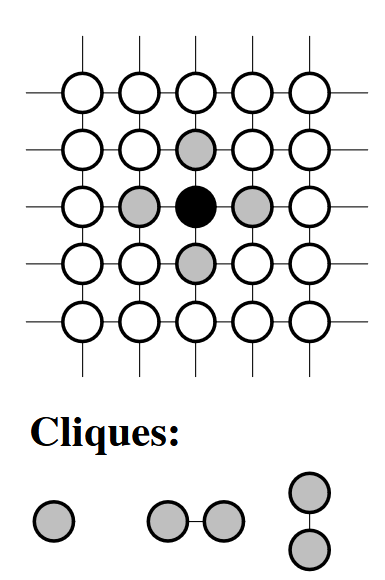
\includegraphics[height=2.5cm]{imgs/article/fig3a_voisinage_ordre1_cliques}%
      \hspace{2mm}%
      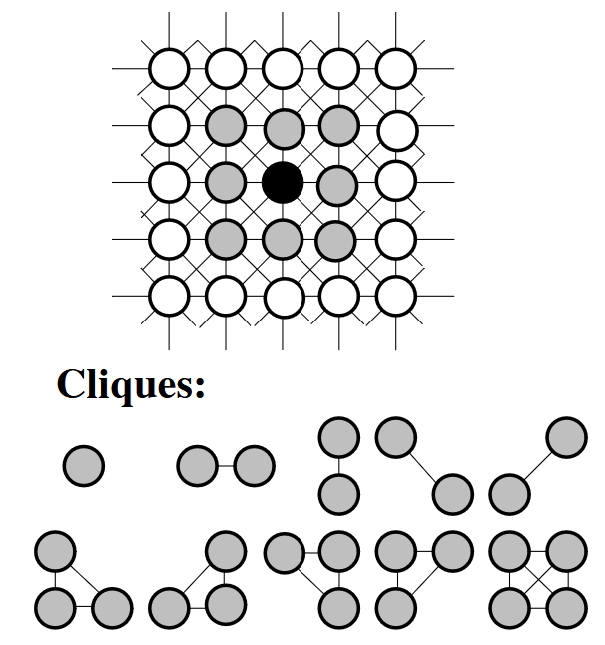
\includegraphics[height=2.5cm]{imgs/article/fig3b_voisinage_ordre2_cliques}
      \legende{(a) 1\textsuperscript{st} order \quad (b) 2\textsuperscript{nd} order}
      \credit{Pixel neighborhoods on a grid and the associated
        cliques \cite{kato2012markov}.}
    \end{column}
  \end{columns}
  \biblio{kato2012markov}
\end{frame}

\begin{frame}{Optimizing: a hard problem}
  \begin{itemize}
    \item Finding the optimal configuration is a hard combinatorial optimization
          problem $\Rightarrow$ \hl{suboptimal} strategies
    \item \hl{Iterated conditional modes (ICM)}, \hl{simulated annealing}\refc{kirkpatrick1984optimization},
          the \hl{Gibbs sampler}\refc{geman1984stochastic}
    \item \hl{Graph cuts}\refc{boykov2001fast}, \hl{loopy belief
          propagation}\refc{tanaka2003loopy}
    \item Application areas: spatial consistency of classifications, multisource
          segmentation, restoration, change detection, optical / radar /
          LiDAR fusion\refc{solberg1996markov}\refc{derin1987modeling}\refc{moser2013combining}
    \item Beyond these applications: a \hl{general probabilistic formulation of
          spatial regularization}
  \end{itemize}
  \biblio{geman1984stochastic,solberg1996markov,kirkpatrick1984optimization,boykov2001fast,tanaka2003loopy,derin1987modeling,moser2013combining}
\end{frame}

\begin{frame}{From MRFs to CRFs}
  \begin{itemize}
    \item Conditional random fields model $P(Y\mid X)$ directly rather than the
          joint distribution\refc{lafferty2001conditional}: this makes
          \hl{complex discriminative features} easier to use
    \item \hl{Fully connected CRFs}: better preserved object
          boundaries\refc{krahenbuhl2011efficient}
    \item Integration into deep networks: refinement modules, \hl{differentiable
          layers}\refc{zheng2015conditional}; hierarchical Markov frameworks and
          learned CRFs\refc{pastorino2021multisensor}\refc{pastorino2022semantic}\refc{pastorino2024crfnet}\refc{voisin2013classification}
    \item \hl{The idea that runs through the field}: a map must be consistent both with
          the local observations \emph{and} with the spatial organization of the scene
  \end{itemize}
  \biblio{lafferty2001conditional,krahenbuhl2011efficient,zheng2015conditional,pastorino2021multisensor,pastorino2022semantic,pastorino2024crfnet,voisin2013classification}
\end{frame}

% ============================================================
\section{Spectral-spatial methods}
% ============================================================
\frame{\sectionpage}

\begin{frame}{Enriching the representation, not the labels}
  \begin{itemize}
    \item Contextual models regularize the \hl{labels}; here the \hl{features} are
          enriched \emph{before} classification\refc{landgrebe2003signal}
    \item Ideas: the \hl{increasing resolution} of sensors, both spatial and spectral
      \begin{itemize}
        \item a single class exhibits strong spectral variability
        \item different objects sometimes have very similar signatures
      \end{itemize}
    \item Texture, shape, size, spatial organization and neighborhood relations become
          \hl{as discriminative as the spectral values
          themselves}\refc{dellepiane1991sar}
  \end{itemize}
  \biblio{landgrebe2003signal,dellepiane1991sar}
\end{frame}

\begin{frame}{Mathematical morphology}
  \begin{columns}[T,onlytextwidth]
    \begin{column}{0.32\textwidth}\centering
      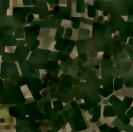
\includegraphics[height=2.25cm]{imgs/article/fig4a_erosion}
      \legende{erosion}
    \end{column}
    \begin{column}{0.32\textwidth}\centering
      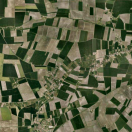
\includegraphics[height=2.25cm]{imgs/article/fig4b_image_originale_rvb}
      \legende{original RGB image}
    \end{column}
    \begin{column}{0.32\textwidth}\centering
      
\includegraphics[height=2.25cm]{imgs/article/fig4c_dilatation}
      \legende{dilation}
    \end{column}
  \end{columns}
  \credit{Erosion (left) and dilation (right) of the original RGB satellite image
    (center).}
  \vspace{0.6ex}
  \begin{itemize}
    \item Local statistics and textural features\refc{haralick1973textural}
    \item \hl{Mathematical morphology} operators: erosion, dilation and their
          compositions\refc{serra1982image}\refc{soille2003morphological}
  \end{itemize}
  \biblio{haralick1973textural,serra1982image,soille2003morphological}
\end{frame}

\begin{frame}{Morphological profiles and attribute profiles}
  \begin{itemize}
    \item \hl{Extended morphological profiles (EMPs)}\refc{benediktsson2005classification} then
          \hl{attribute profiles}\refc{dallamura2010morphological}: describing spectral
          properties and spatial structure simultaneously \hl{at several scales}
    \item Reference methods for hyperspectral data and very high resolution
    \item Combined with SVMs: remarkable performance\refc{campsvalls2009kernel}\refc{fauvel2008spectral},
          but the principle is general (random forests, neural networks\dots)
    \item Dimensionality reduction, subspace-based methods, multisource
          data fusion\refc{plaza2009recent}\refc{campsvalls2014advances}
    \item Using \hl{segmented regions} rather than pixels as analysis units: greater
          spatial consistency, less noise\refc{tarabalka2009spectral}
  \end{itemize}
  \biblio{campsvalls2009kernel,benediktsson2005classification,dallamura2010morphological,fauvel2008spectral,plaza2009recent,campsvalls2014advances,tarabalka2009spectral}
\end{frame}

% ============================================================
\section{Variational methods}
% ============================================================
\frame{\sectionpage}

\begin{frame}{Segmenting by minimizing an energy}
  \begin{itemize}
    \item Late 1980s, in parallel with Markov random fields: \hl{no explicit probability
          distribution on the labels}, but the \hl{search for the partition}
          achieving the best trade-off between \hl{fidelity to the observations} and
          \hl{regularity}\refc{kato2012markov}\refc{mumford1989optimal}\refc{samson2000variational}
    \item \hl{Active contours}: boundaries are deformable curves evolving under the
          action\refc{samson2000variational}\refc{kass1988snakes}
      \begin{itemize}
        \item of \emph{internal forces} (contour regularity)
        \item of \emph{external forces} (derived from the image information)
      \end{itemize}
    \item An \hl{explicit} representation of contours, and the starting point of a
          large family of energy-minimization methods
  \end{itemize}
  \biblio{kato2012markov,mumford1989optimal,samson2000variational,kass1988snakes}
\end{frame}

\begin{frame}{The Mumford--Shah functional}
  \formulebox[0.96]{$\displaystyle E(u,K) \;=\;
     \underbrace{\int_{\Omega} (u - I)^2\,\mathrm{d}x}
                _{\textcolor{inria-rouge}{\text{\scriptsize data fidelity}}}
     \;+\; \mu \underbrace{\int_{\Omega \setminus K} |\nabla u|^2\,\mathrm{d}x}
                _{\textcolor{inria-rouge}{\text{\scriptsize within-region smoothness}}}
     \;+\; \nu\, \underbrace{|K|\vphantom{\int}}
                _{\textcolor{inria-rouge}{\text{\scriptsize boundary complexity}}}$}
  \begin{itemize}
    \item $u$: the reconstructed image, $I$: the observed image, $K$: the set of
          discontinuities (the boundaries)\refc{mumford1989optimal}
    \item $\mu > 0$: smoothness of the solution inside the regions;
          $\nu > 0$: weight of the boundary measure
    \item An explicit trade-off between \hl{data fit} and
          \hl{regularity of the solution}, a principle shared by many segmentation
          methods
    \item One of the most influential variational models in image processing
  \end{itemize}
  \biblio{mumford1989optimal}
\end{frame}

\begin{frame}{Numerical robustness and applications}
  \begin{columns}[T,onlytextwidth]
    \begin{column}{0.60\textwidth}
      \begin{itemize}
        \item \hl{Level sets}: contours represented implicitly, topology changes
              handled automatically\refc{osher1988fronts}
        \item \hl{Region-based models}: region statistics rather than gradients
              alone, robust to noise and low
              contrast\refc{chan2001active}
        \item In remote sensing: \hl{high-resolution optical segmentation},
              \hl{restoration}, \hl{fusion}, \hl{object extraction};
              \hl{classification and restoration} unified in a single
              functional\refc{samson2000variational}
      \end{itemize}
    \end{column}
    \begin{column}{0.38\textwidth}\centering
      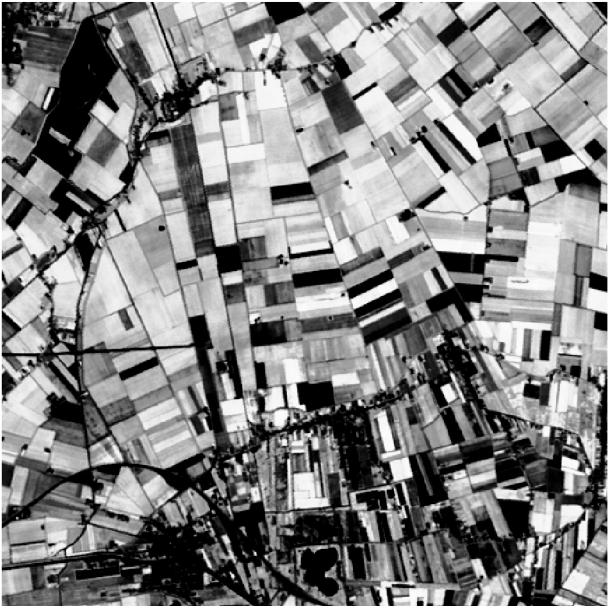
\includegraphics[width=0.485\textwidth]{imgs/article/fig5a_spot_cnes}%
      \hspace{1mm}%
      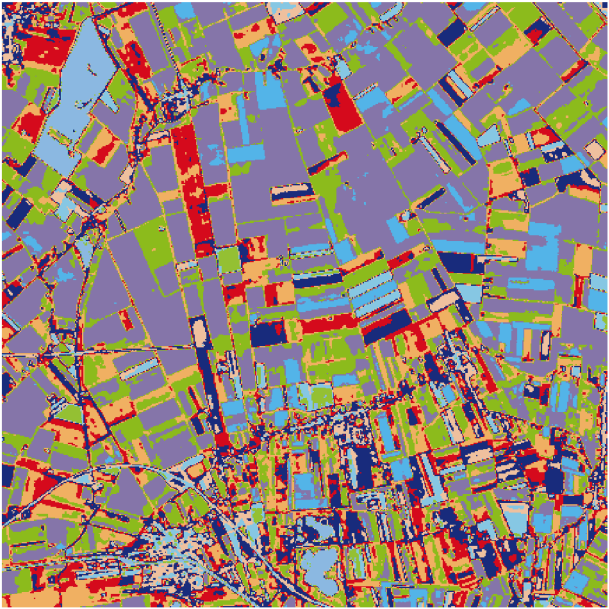
\includegraphics[width=0.485\textwidth]{imgs/article/fig5b_segmentation_variationnelle}
      \legende{(a) SPOT image \quad (b) segmentation}
      \credit{(a) SPOT satellite image \copyright{} CNES; (b) segmentation by the
        variational method of \cite{samson2000variational}.}
    \end{column}
  \end{columns}
  \vspace{0.6ex}
  \begin{itemize}
    \item \hl{Convergence}: Bayesian, Markov random field, variational and
          graph-based formulations are different expressions of the same
          principle: \hl{data term $+$ regularization}
  \end{itemize}
  \biblio{samson2000variational,osher1988fronts,chan2001active}
\end{frame}

% ============================================================
\section{Deep learning}
% ============================================================
\frame{\sectionpage}

\begin{frame}{2012, the turning point}
  \begin{itemize}
    \item \hl{AlexNet} demonstrates a dramatic improvement in natural-image
          classification\refc{krizhevsky2012imagenet}
    \item \hl{Learning} \hl{hierarchical representations} directly from the data,
          without hand-crafted design of spectral, textural or geometric
          features
    \item Performance now depends on the ability of the network to learn
          \hl{jointly} a relevant representation \emph{and} the decision
          function
    \item Rapid adoption in remote sensing: more discriminative
          representations, \hl{transfer} of models pretrained on large datasets
          of natural images\refc{chen2014deep}\refc{castelluccio2015land}
    \item \hl{Spectral-spatial approaches} shift from \emph{hand-crafted} to
          \emph{learned} representations
  \end{itemize}
  \biblio{krizhevsky2012imagenet,chen2014deep,castelluccio2015land}
\end{frame}

\begin{frame}{Dense prediction: FCNs and encoder--decoder}
  \begin{columns}[T,onlytextwidth]
    \begin{column}{0.55\textwidth}
      \begin{itemize}
        \item \hl{FCNs}: fully connected layers replaced by convolutional
              operations $\Rightarrow$ dense, pixel-level prediction, learned
              end-to-end\refc{long2015fully}
        \item \hl{U-Net}: an encoder--decoder whose \emph{skip connections}
              restore the localization lost in downsampling, hence better
              boundaries and smaller objects\refc{ronneberger2015unet}
        \item \hl{Applications}: land cover, buildings, roads, hydrographic
              networks\refc{audebert2018beyond}\refc{zhang2018road}\refc{isikdogan2017surface}
      \end{itemize}
    \end{column}
    \begin{column}{0.43\textwidth}\centering
      \vspace{0.4cm}
      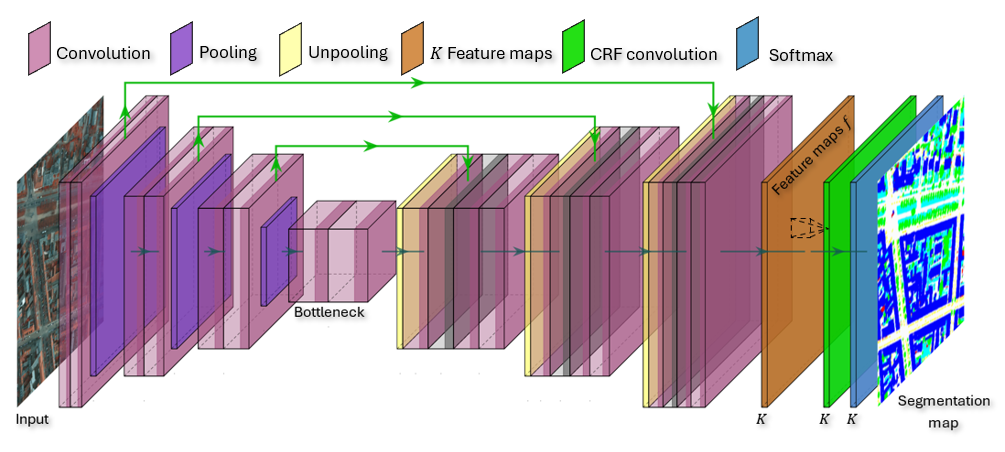
\includegraphics[width=\textwidth]{imgs/article/fig6_fcn_potsdam}
      \legende{FCN architecture}
      \credit{Applied to the aerial images of the ISPRS \emph{2D Semantic
        Labeling Challenge} dataset (Potsdam) \cite{pastorino2026probabilistic}.}
    \end{column}
  \end{columns}
  \biblio{long2015fully,pastorino2026probabilistic,ronneberger2015unet,audebert2018beyond,zhang2018road,isikdogan2017surface}
\end{frame}

\begin{frame}{Context, scales, modalities}
  \begin{itemize}
    \item \hl{Residual networks}: learning deeper models while limiting the
          vanishing gradient\refc{he2016deep}
    \item \hl{DeepLab}: dilated convolutions and multiscale aggregation (Atrous Spatial
          Pyramid Pooling, ASPP) to enlarge the receptive field \emph{without} degrading
          the resolution of the predictions\refc{chen2017rethinking}\refc{chen2018encoder}
    \item \hl{Feature pyramids}: objects of widely varying
          sizes\refc{lin2017feature}, decisive in remote sensing where a single scene
          contains vehicles, buildings, fields and forest stands
    \item \hl{Multimodality}: learning shared representations from optical, SAR and
          LiDAR data, digital terrain models and ancillary geospatial
          data\refc{audebert2018beyond}\refc{ma2019deep}
  \end{itemize}
  \biblio{audebert2018beyond,he2016deep,chen2017rethinking,chen2018encoder,lin2017feature,ma2019deep}
\end{frame}

\begin{frame}{What deep learning does not eliminate}
  \begin{itemize}
    \item Spatial context, multiscale representation, data fusion, object hierarchy:
          \hl{reformulated} within an end-to-end learning framework, not
          abandoned
    \item Persistent limitations of convolutional networks:
      \begin{itemize}
        \item pixel-level annotations are \hl{costly}, particularly in remote sensing
        \item limited \hl{generalization} across sensors, geographical regions and
              acquisition modalities
        \item difficulty in modeling \hl{very long-range} spatial dependencies
      \end{itemize}
    \item These limitations pave the way for \hl{attention mechanisms}, and then for
          \hl{geospatial foundation models}
  \end{itemize}
\end{frame}

% ============================================================
\section{Transformers and foundation models}
% ============================================================
\frame{\sectionpage}

\begin{frame}{Attention in segmentation}
  \begin{itemize}
    \item Developed for language processing, transformers directly model the relations
          between \hl{distant elements} of a
          sequence\refc{vaswani2017attention}; their adaptation to vision opens a
          new phase\refc{dosovitskiy2021image}
    \item \hl{Swin Transformer}\refc{liu2021swin} and \hl{SegFormer}\refc{xie2021segformer}:
          combining a \emph{hierarchical} representation of the image with a
          \emph{global} modeling of the context
    \item Particularly relevant in remote sensing: identifying a building,
          a road or a field does not rely on local appearance alone,
          but on its \hl{organization within the scene}
  \end{itemize}
  \biblio{vaswani2017attention,dosovitskiy2021image,liu2021swin,xie2021segformer}
\end{frame}

\begin{frame}{Learning without annotations}
  \begin{itemize}
    \item \hl{Self-supervised learning} becomes a major research direction
    \item \hl{Masked autoencoders} show that rich visual representations can be
          learned from large amounts of \hl{unlabeled}
          data\refc{he2022masked}
    \item A direct response to an \hl{imbalance} specific to the field:
      \begin{itemize}
        \item satellite archives are \hl{abundant}
        \item pixel-level annotations remain \hl{scarce and costly}
      \end{itemize}
  \end{itemize}
  \biblio{he2022masked}
\end{frame}

\begin{frame}{Geospatial foundation models}
  \begin{columns}[T,onlytextwidth]
    \begin{column}{0.52\textwidth}
      \begin{itemize}
        \item \hl{Pretrained on very large volumes of data}, then adapted:
              classification, segmentation, object detection and change
              detection\refc{brown2025alphaearth}\refc{cong2022satmae}\refc{jakubik2023foundation}\refc{wang2023empirical}\refc{kirillov2023segment}
        \item The goal: \hl{generic representations}, \hl{transferable} across
              sensors, geographical regions and applications
        \item The \hl{cost} of pretraining (compute, energy) $\Rightarrow$ environmental
              footprint and accessibility
      \end{itemize}
    \end{column}
    \begin{column}{0.46\textwidth}\centering
      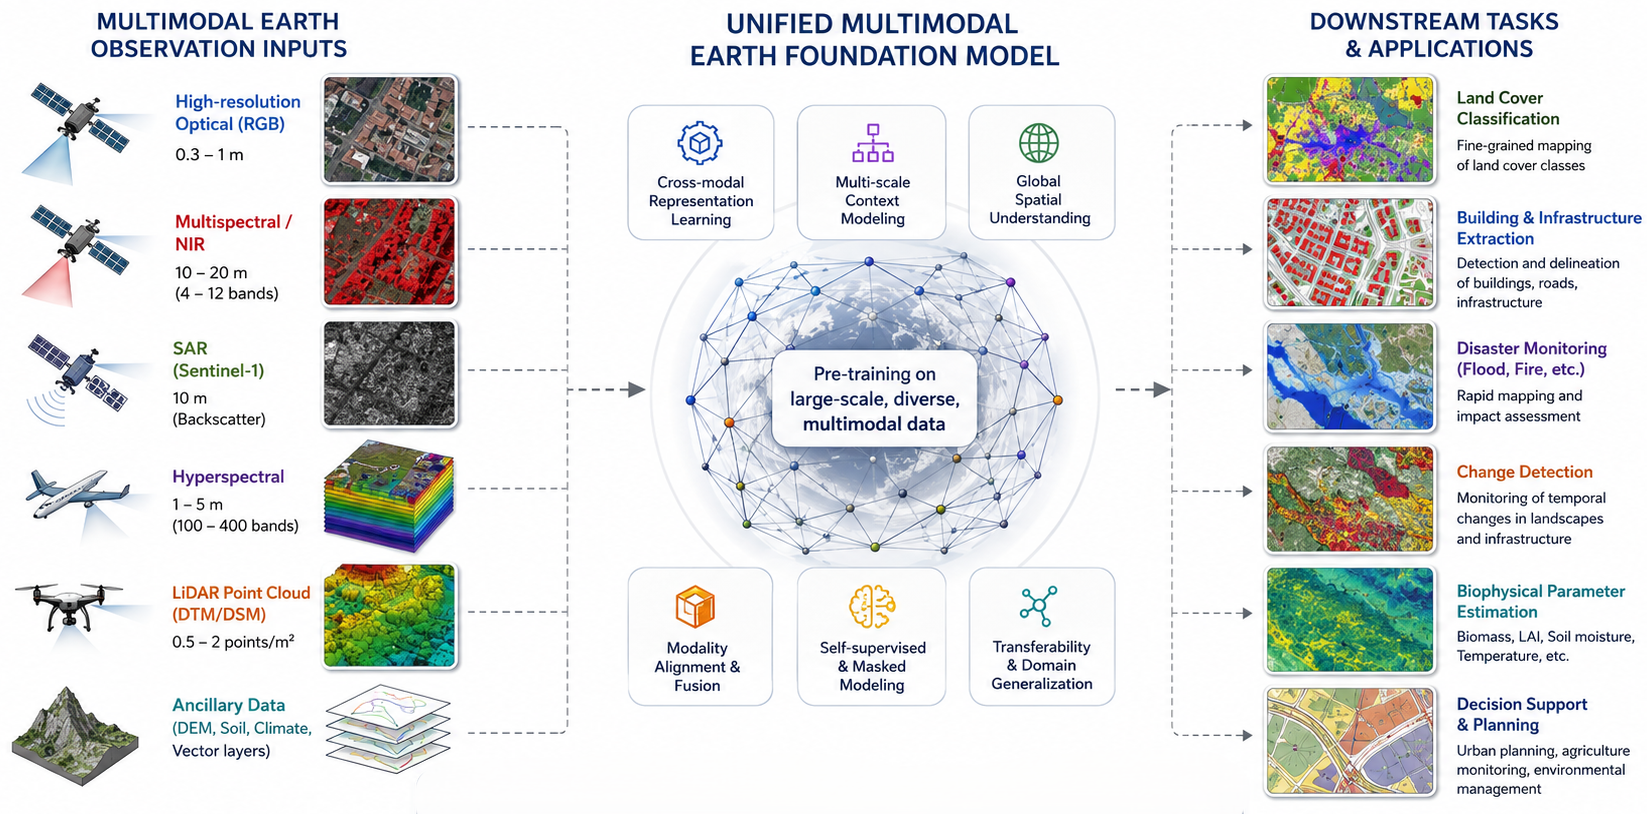
\includegraphics[width=\textwidth]{imgs/article/fig7_modele_fondation_geospatial}
      \legende{general principle of a geospatial foundation model}
    \end{column}
  \end{columns}
  \vspace{0.4ex}
  \begin{itemize}
    \item Not a break: the same questions (heterogeneity, context, generalization)
          are now \hl{learned} rather than \hl{hand-crafted}
  \end{itemize}
  \biblio{brown2025alphaearth,cong2022satmae,jakubik2023foundation,wang2023empirical,kirillov2023segment}
\end{frame}

% ============================================================
\section{Conclusion}
% ============================================================
\frame{\sectionpage}

\begin{frame}{A nonlinear history}
  \begin{itemize}
    \item Not a simple trajectory from statistical classifiers to deep networks, but
          the \hl{convergence of several families of methods}: statistical
          classification, kernel methods, ensemble methods, contextual models,
          Markov random fields, variational methods, stochastic geometry, deep
          learning, foundation models
    \item One unifying reading: the \hl{progressive integration of increasing levels of
          context}
  \end{itemize}
  \vspace{0.6ex}
  \filrouge
  \vspace{0.4ex}
  \begin{itemize}
    \item One recurring principle: \hl{data term $+$ regularization},
          from Markov random fields to the loss functions of deep networks
  \end{itemize}
\end{frame}

\begin{frame}{Outlook}
  \begin{columns}[T,onlytextwidth]
    \begin{column}{0.48\textwidth}
      \begin{itemize}
        \item Geographic generalization
        \item Lack of annotations
        \item Optical, radar and LiDAR fusion
      \end{itemize}
    \end{column}
    \begin{column}{0.48\textwidth}
      \begin{itemize}
        \item Accounting for the temporal dimension
        \item Model interpretability
        \item Operational robustness
      \end{itemize}
    \end{column}
  \end{columns}
  \vspace{1.2ex}
  \begin{itemize}
    \item Semantic segmentation in remote sensing remains an \hl{open field},
          at the intersection of signal and image processing, probabilistic
          modeling, geometry, computer vision and artificial intelligence,
          in a geospatial setting
  \end{itemize}
\end{frame}

% ---- Thank you ---------------------------------------------
\frame{\merci}

% ============================================================
% Appendix: references then figure credits
% ============================================================
\begin{frame}[allowframebreaks]{References}
  \printbibliography[heading=none]
\end{frame}

\begin{frame}{Figure credits}
  \vspace{1ex}
  \begin{itemize}\footnotesize
    \item Aerial image and segmentation map: \emph{Zeebruges} dataset,
      IEEE GRSS Image Analysis and Data Fusion (IADF) Technical Committee;
      imagery and ground-truth data provided by the Belgian Royal Military Academy
      and ONERA (the French Aerospace Lab).
    \item IKONOS satellite image, 4~m, 3 bands, false-color composite
      (near infrared, red, blue); per-pixel and contextual segmentation
      maps \cite{moser2013landcover}.
    \item First- and second-order neighborhoods on a grid, and the associated
      cliques \cite{kato2012markov}.
    \item Erosion and dilation of an RGB satellite image.
    \item SPOT satellite image \copyright{} CNES; segmentation map obtained with
      the variational method of \cite{samson2000variational}.
    \item Architecture of an FCN applied to the aerial images of the ISPRS
      \emph{2D Semantic Labeling Challenge} dataset (Potsdam) \cite{pastorino2026probabilistic}.
    \item General principle of a geospatial foundation model.
  \end{itemize}
  \biblio{moser2013landcover,kato2012markov,samson2000variational,pastorino2026probabilistic}
\end{frame}

\end{document}
